\documentclass[12pt]{article}
\usepackage{amsmath, amsfonts}
\usepackage{hyperref}
\usepackage[font=large,labelfont=bf]{caption}
\usepackage{tikz, pgfplots}
\pgfplotsset{compat=newest}
\usetikzlibrary{positioning, arrows.meta, quotes}
\usetikzlibrary{shapes, snakes}
\usepackage{geometry}
 \geometry{
 a4paper,
 total={170mm,257mm},
 left=30mm,right=30mm,
 top=20mm,
 }
\title{Intuitive Understanding of Newton-Raphson Method}
\author{Xinyu Chen}

\begin{document}
\large
\maketitle

\begin{abstract}
Newton-Raphson method is a classical and powerful algorithm for numerically determining the root of some equations. This post will introduce some simple and intuitive examples for showing how does the Newton-Raphson method work for finding the root of equations.
\end{abstract}

\section{Start with a Quadratic Equation}

Quadratic equation is one of the most classical equation in math, which takes the form of $ax^2+bx+c=0$. If we have a quadratic equation $x^2-4=0$, then as we know, the positive solution is $x=2$.

For graphical convenience, we define a function as $f(x)=x^2-4$. The derivative of the function is $f^\prime(x)=2x$.

\begin{figure}[h]
    \centering
    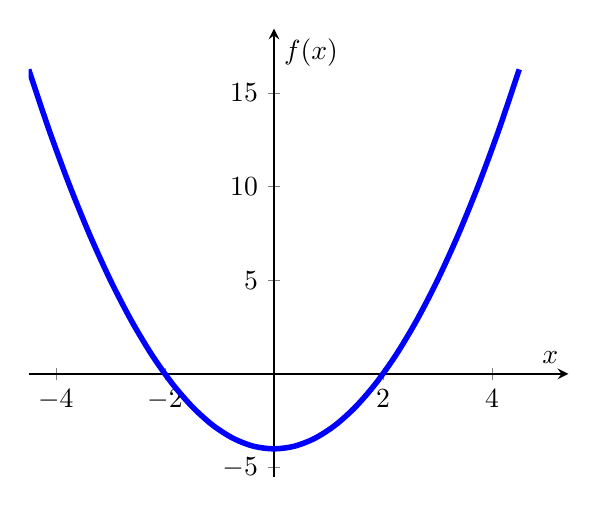
\begin{tikzpicture}
\begin{axis}[axis lines=middle, line width=0.7, enlargelimits=upper, domain=-4.5:4.5, ymin=-5.5, xlabel=$x$, ylabel=$f(x)$]
\addplot [smooth, color=blue, line width = 2] {x^2-4};
\end{axis}
\end{tikzpicture}
    \caption{{\color{blue}$f(x)=x^2-4$} (blue curve).}
    \label{example1_s1}
\end{figure}

\clearpage

If we use $x_0=4$ as starting point, then $(4,12)$ is the point of intersection.

\begin{figure}[h]
    \centering
    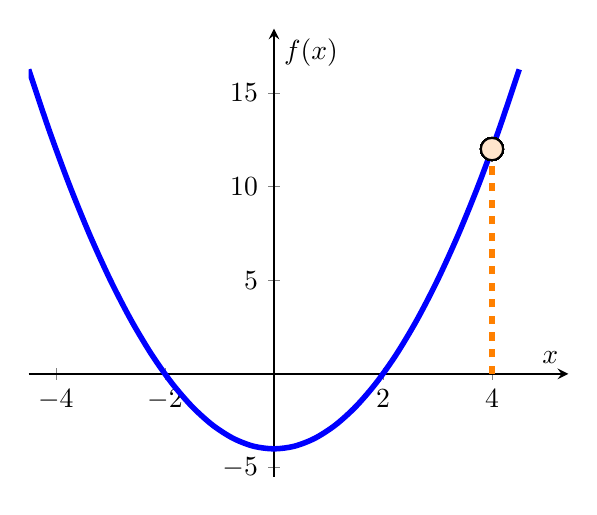
\begin{tikzpicture}
\begin{axis}[axis lines=middle, line width=0.7, enlargelimits=upper, domain=-4.5:4.5, ymin=-5.5, xlabel=$x$, ylabel=$f(x)$]
\addplot [smooth, color=blue, line width = 2] {x^2-4};
\addplot[smooth, color=orange, dashed, line width = 2] coordinates {(4,0) (4,12)};
\addplot[only marks, mark size=4, color=orange!20, draw=black] (4,12);
\end{axis}
\end{tikzpicture}
    \caption{{\color{blue}$f(x)=x^2-4$} (blue curve); {\color{orange}$x=4$} (dashed orange line); {\color{orange}$(4,12)$} (orange dot).}
    \label{example1_s2}
\end{figure}

For the point $(4,12)$, the tangent line is $f(x)=8x-20$.

\begin{figure}[h]
    \centering
    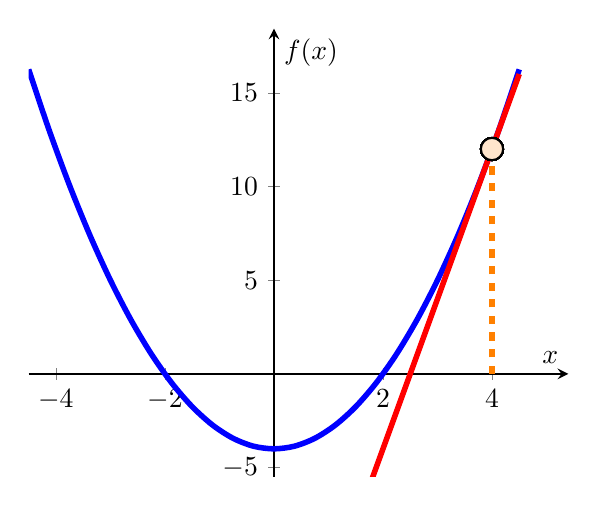
\begin{tikzpicture}
\begin{axis}[axis lines=middle, line width=0.7, enlargelimits=upper, domain=-4.5:4.5, ymin=-5.5, xlabel=$x$, ylabel=$f(x)$]
\addplot [smooth, color=blue, line width = 2] {x^2-4};
\addplot[smooth, color=orange, dashed, line width = 2] coordinates {(4,0) (4,12)};
\addplot[only marks, mark size=4, color=orange!20, draw=black] (4,12);
\addplot [smooth, color=red, line width = 2] {8*x-20};
\end{axis}
\end{tikzpicture}
    \caption{{\color{blue}$f(x)=x^2-4$} (blue curve); {\color{orange}$x=4$} (dashed orange line); {\color{orange}$(4,12)$} (orange dot); {\color{red}$y=8x-20$} (red line).}
    \label{example1_s3}
\end{figure}

\clearpage

The point of intersection of tangent line and $x$ axis is $(\frac{5}{2},0)$. If we use $x_1=\frac{5}{2}$ as a new point, then $(\frac{5}{2},\frac{9}{4})$ is the point of intersection.

\begin{figure}[h]
    \centering
    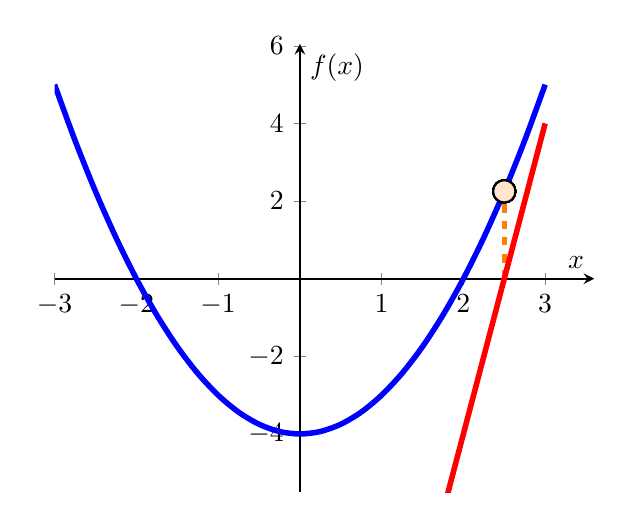
\begin{tikzpicture}
\begin{axis}[axis lines=middle, line width=0.7, enlargelimits=upper, domain=-3:3, ymin=-5.5, xlabel=$x$, ylabel=$f(x)$]
\addplot [smooth, color=blue, line width = 2] {x^2-4};
\addplot[smooth, color=orange, dashed, line width = 2] coordinates {(2.5,0) (2.5,2.25)};
\addplot[only marks, mark size=4, color=orange!20, draw=black] (2.5,2.25);
\addplot [smooth, color=red, line width = 2] {8*x-20};
\end{axis}
\end{tikzpicture}
    \caption{{\color{blue}$f(x)=x^2-4$} (blue curve); {\color{orange}$x=\frac{5}{2}$} (dashed orange line); {\color{orange}$(\frac{5}{2},\frac{9}{4})$} (orange dot); {\color{red}$y=8x-20$} (red line).}
    \label{example1_s4}
\end{figure}

For the point $(\frac{5}{2},\frac{9}{4})$, the tangent line is $f(x)=5x-\frac{41}{4}$.

\begin{figure}[h]
    \centering
    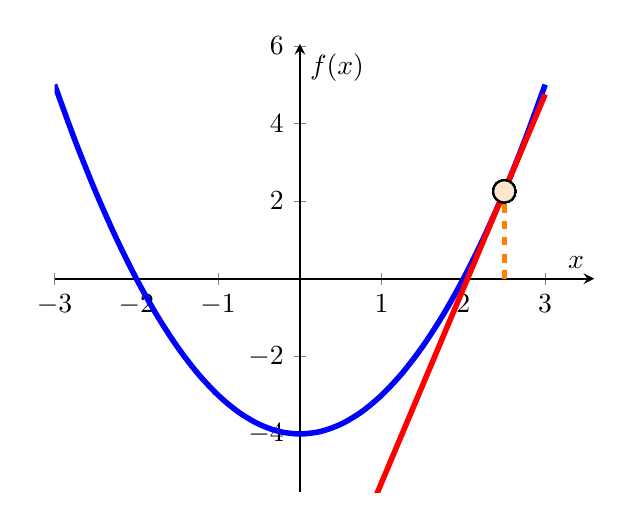
\begin{tikzpicture}
\begin{axis}[axis lines=middle, line width=0.7, enlargelimits=upper, domain=-3:3, ymin=-5.5, xlabel=$x$, ylabel=$f(x)$]
\addplot [smooth, color=blue, line width = 2] {x^2-4};
\addplot[smooth, color=orange, dashed, line width = 2] coordinates {(2.5,0) (2.5,2.25)};
\addplot[only marks, mark size=4, color=orange!20, draw=black] (2.5,2.25);
\addplot [smooth, color=red, line width = 2] {5*x-41/4};
\end{axis}
\end{tikzpicture}
    \caption{{\color{blue}$f(x)=x^2-4$} (blue curve); {\color{orange}$x=\frac{5}{2}$} (dashed orange line); {\color{orange}$(\frac{5}{2},\frac{9}{4})$} (orange dot); {\color{red}$y=5x-\frac{41}{4}$} (red line).}
    \label{example1_s5}
\end{figure}

The point of intersection of tangent line and $x$ axis is $(\frac{41}{20},0)$. As can be seen, the $x$ coordinate $\frac{41}{20}=2.05$ is very close to the solution $x=2$.

\clearpage

\section{Revisit Newton's Motivation}

In the rather early stage, Newton tried to motivate the idea using equation $x^3-2x-5=0$. As we know, the solution is very close to 2. Perhaps, we can try to use $x_0=2$ as starting point.

\begin{figure}[h]
    \centering
    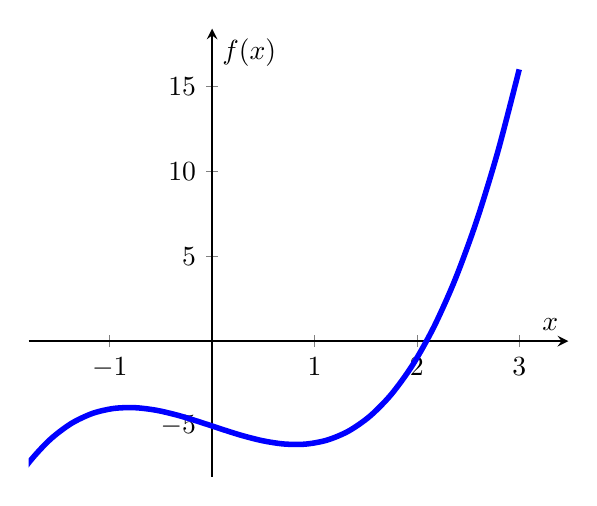
\begin{tikzpicture}
\begin{axis}[axis lines=middle, line width=0.7, enlargelimits=upper, domain=-2:3, ymin=-8, xlabel=$x$, ylabel=$f(x)$]
\addplot [smooth, color=blue, line width = 2] {x^3-2*x-5};
\end{axis}
\end{tikzpicture}
    \caption{{\color{blue}$f(x)=x^3-2x-5$} (blue curve).}
    \label{example2_s1}
\end{figure}

Recall that $f^\prime(x)=3x^2-2$.
\begin{enumerate}
\item Use $x_0=2$, then $(x_0,f(x_0))=(2,-1)$ and $f^\prime(x_0)=10$.
\item Tangent line is $f(x)=10x-21$, and the point of intersection of tangent line and $x$ axis is $(2.1,0)$.
\item Use $x_1=2.1$, then $(x_1,f(x_1))=(2.1,0.061)$ and $f^\prime(x_1)=11.23$.
\item Tangent line is $f(x)=11.23x-23.522$, and the point of intersection of tangent line and $x$ axis is $(2.094568,0)$.
\end{enumerate}

Note that $x_2=2.094568$ is very close to the final estimate achieved by Newton, i.e., $x=2.09455148$.

\clearpage

\section{Explain Newton-Raphson Iteration}

For any equation $f(x)=0$, the Newton-Raphson iteration is
\begin{equation*}
x_{n+1}=x_{n}-\frac{f(x_{n})}{f^\prime(x_{n})}
\end{equation*}

Suppose $x^3-2x^2-11x+12=0$, how to use the Newton-Raphson iteration to obtain the solution with the starting point $x_0=2$?

\begin{figure}[h]
    \centering
    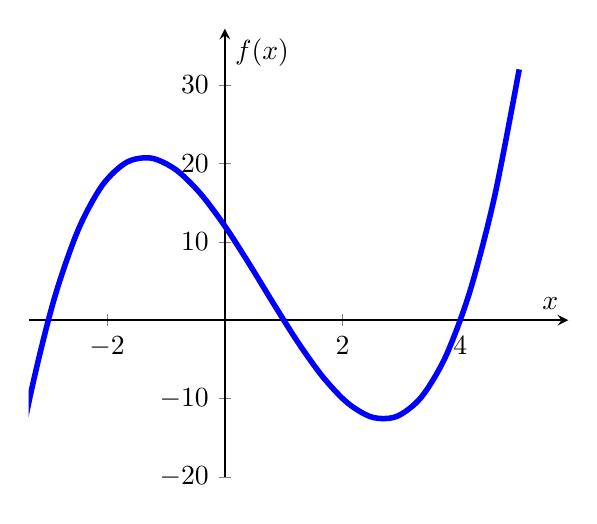
\begin{tikzpicture}
\begin{axis}[axis lines=middle, line width=0.7, enlargelimits=upper,ymin=-20, xlabel=$x$, ylabel=$f(x)$]
\addplot [smooth, color=blue, line width = 2] {x^3-2*x^2-11*x+12};
\end{axis}
\end{tikzpicture}
    \caption{{\color{blue}$f(x)=x^3-2x^2-11x+12$} (blue curve).}
\end{figure}

Note that $f^\prime(x)=3x^2-4x-11$.

If $x_0=2$, then
\begin{equation*}
x_1=x_{0}-\frac{f(x_{0})}{f^\prime(x_{0})}=2-\frac{f(2)}{f^\prime(2)}=0.5714285714285714
\end{equation*}

\begin{figure}[h]
    \centering
    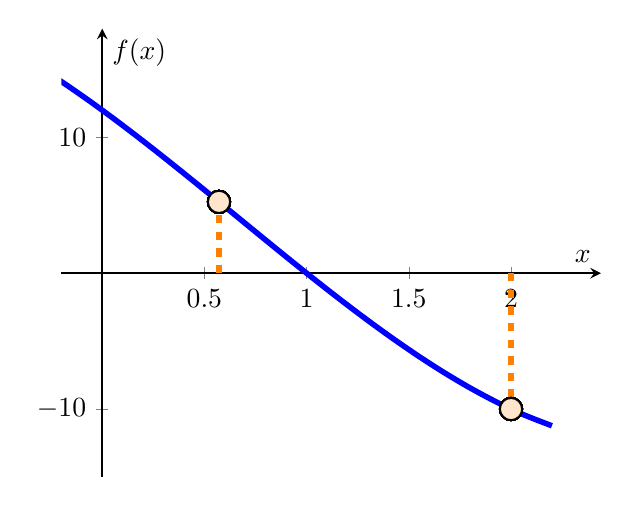
\begin{tikzpicture}
\begin{axis}[axis lines=middle, line width=0.7, enlargelimits=upper, domain=-1:2.2, ymax=15, ymin=-15, xlabel=$x$, ylabel=$f(x)$]
\addplot [smooth, color=blue, line width = 2] {x^3-2*x^2-11*x+12};
\addplot[smooth, color=orange, dashed, line width = 2] coordinates {(2,0) (2,-10)};
\addplot[only marks, mark size=4, color=orange!20, draw=black] (2,-10);
\addplot[smooth, color=orange, dashed, line width = 2] coordinates {(0.5714285714285714,0) (0.5714285714285714,5.247813411078718)};
\addplot[only marks, mark size=4, color=orange!20, draw=black] (0.5714285714285714,5.247813411078718);
\end{axis}
\end{tikzpicture}
    \caption{{\color{blue}$f(x)=x^3-2x^2-11x+12$} (blue curve); {\color{orange}$x_0=2,x_1=0.57143$} (orange line).}
\end{figure}

\clearpage

As $x_1=0.5714285714285714$, then
\begin{equation*}
x_2=x_{1}-\frac{f(x_{1})}{f^\prime(x_{1})}=0.9978678038379531
\end{equation*}

\begin{figure}[h]
    \centering
    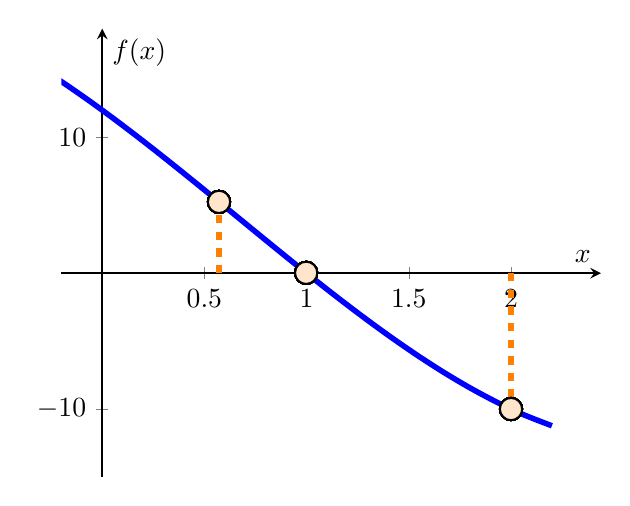
\begin{tikzpicture}
\begin{axis}[axis lines=middle, line width=0.7, enlargelimits=upper, domain=-1:2.2, ymax=15, ymin=-15, xlabel=$x$, ylabel=$f(x)$]
\addplot [smooth, color=blue, line width = 2] {x^3-2*x^2-11*x+12};
\addplot[smooth, color=orange, dashed, line width = 2] coordinates {(2,0) (2,-10)};
\addplot[only marks, mark size=4, color=orange!20, draw=black] (2,-10);
\addplot[smooth, color=orange, dashed, line width = 2] coordinates {(0.5714285714285714,0) (0.5714285714285714,5.247813411078718)};
\addplot[only marks, mark size=4, color=orange!20, draw=black] (0.5714285714285714,5.247813411078718);
\addplot[smooth, color=orange, dashed, line width = 2] coordinates {(0.9978678038379531,0) (0.9978678038379531,0.025590890511516307)};
\addplot[only marks, mark size=4, color=orange!20, draw=black] (0.9978678038379531,0.025590890511516307);
\end{axis}
\end{tikzpicture}
    \caption{{\color{blue}$f(x)=x^3-2x^2-11x+12$} (blue curve); {\color{orange}$x_0=2,x_1=0.57143,x_2=0.99787$} (orange line).}
\end{figure}

\end{document}
